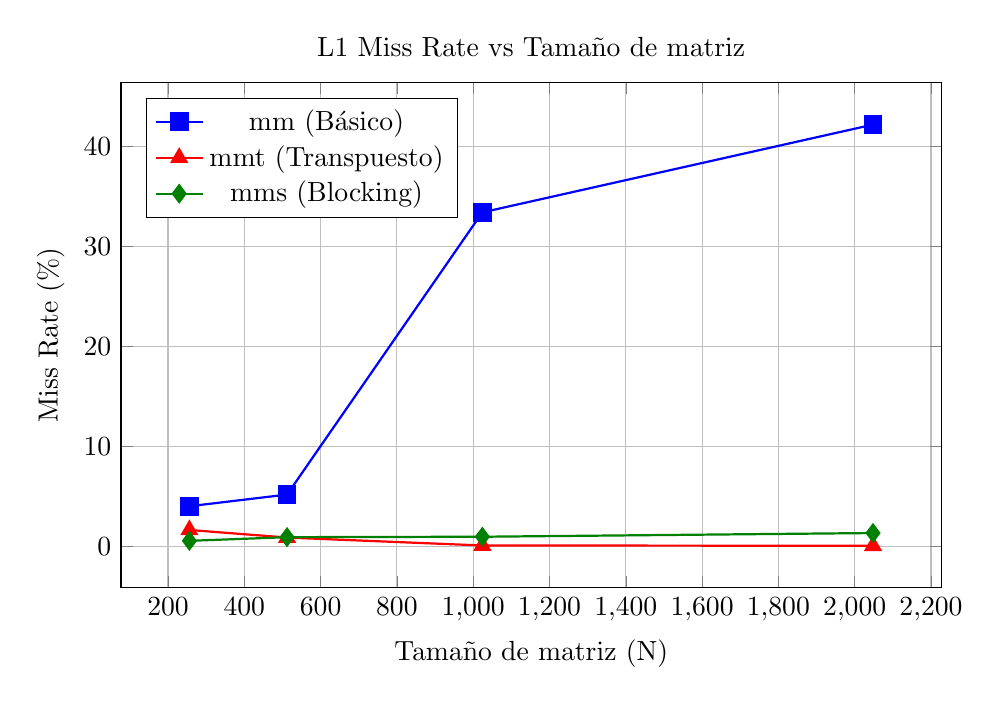
\begin{tikzpicture}
    \begin{axis}[
        title={L1 Miss Rate vs Tamaño de matriz},
        xlabel={Tamaño de matriz (N)},
        ylabel={Miss Rate (\%)},
        legend pos=north west,
        grid=major,
        width=12cm,
        height=8cm,
    ]
        \addplot[
            color=blue,
            mark=square*,
            thick,
            mark size=3pt,
        ]
        coordinates {
            (256, 4.0488)
            (512, 5.2124)
            (1024, 33.4001)
            (2048, 42.1655)
        };
        \addlegendentry{mm (Básico)}
        \addplot[
            color=red,
            mark=triangle*,
            thick,
            mark size=3pt,
        ]
        coordinates {
            (256, 1.6783)
            (512, 0.9185)
            (1024, 0.1262)
            (2048, 0.1)
        };
        \addlegendentry{mmt (Transpuesto)}
        \addplot[
            color=green!50!black,
            mark=diamond*,
            thick,
            mark size=3pt,
        ]
        coordinates {
            (256, 0.5917)
            (512, 0.9573)
            (1024, 1.0005)
            (2048, 1.3714)
        };
        \addlegendentry{mms (Blocking)}
    \end{axis}
\end{tikzpicture}

